\documentclass{beamer}

\usepackage{tikz}
\usetikzlibrary{positioning,matrix, arrows.meta}
\usetikzlibrary{graphdrawing.trees}
\usetikzlibrary{external}
\tikzexternalize % activate!
\usepackage{color}
\newcommand{\vet}[1]{\foreach \num in {#1}{\el{\num}}}
\newcommand{\vetempty}[1]{\foreach \num in {#1}{\elempty{\num}}}
\newcommand{\el}[1]{\tikz{\node[font=\smaller, draw]{#1}}}
\newcommand{\elempty}[1]{\tikz{\node[font=\small, minimum size=1cm, draw=white, fill=white]{#1}}}
\newcommand{\bl}{\color{blue}}
\newcommand{\gr}{\color{gray}}
\newcommand{\re}{\color{red}}
\newcommand{\tcb}[1]{\textcolor{blue}{#1}}
\newcommand{\tcg}[1]{\textcolor{green}{#1}}
\newcommand{\tcr}[1]{\textcolor{red}{#1}}
\newcommand{\ar}{\tikz{\draw [->] (0,0) -- (0,0.4)}}
\newcommand{\nd}{\color{white!0}.}

\usepackage{beamerthemeSingapore}
\usepackage{graphicx}
%\usepackage{here}
\usepackage{url}
\usepackage[brazil]{babel}
\usepackage[T1]{fontenc}
\usepackage[utf8]{inputenc}
%\usepackage[tight,raggedright]{subfigure}
\usepackage{subfigure}
\usepackage[alf]{abntex2cite}
\usepackage{listings}
\usepackage{minted}
\usepackage[linesnumbered,ruled,vlined]{algorithm2e}
\usepackage{amsmath}
\usepackage{pdfpages}
% Please add the following required packages to your document preamble:
\usepackage{booktabs}
\usepackage{ragged2e}
\usepackage{etoolbox}
\usepackage{mathtools}
\usepackage{caption}
\usepackage{xmpmulti}
\usepackage[usestackEOL]{stackengine}
\edef\tmp{\the\baselineskip}
\setstackgap{L}{\tmp}

\DeclareTextFontCommand{\textbf}{\bfseries}
\DeclareTextFontCommand{\textit}{\itshape}

\tikzset{
  treenode/.style = {align=center, inner sep=0pt, text centered,
    font=\sffamily},
  arn_bf/.style = {treenode, rectangle, rounded corners=.8ex, black, font=\sffamily\bfseries, draw=black,fill=white, text width=3.5em, inner sep=2pt },% arbre rouge noir, noeud noir
  arn_rf/.style = {treenode, rectangle, rounded corners=.8ex, red, font=\sffamily\bfseries, draw=red,fill=white, text width=3.5em, inner sep=2pt },% arbre rouge noir, noeud noir
  arn_bt/.style = {treenode, rectangle, rounded corners=.8ex, black, font=\sffamily\bfseries, draw=black,fill=white, text width=2.5em, inner sep=2pt },% arbre rouge noir, noeud noir
  arn_rt/.style = {treenode, rectangle, rounded corners=.8ex, red, font=\sffamily\bfseries, draw=red,fill=white, text width=2.5em, inner sep=2pt },% arbre rouge noir, noeud noir
  arn_b/.style = {treenode, circle, black, font=\sffamily\bfseries, draw=black,
    fill=white, text width=1.5em},% arbre rouge noir, noeud noir
  arn_bl/.style = {treenode, circle, blue, font=\sffamily\bfseries, draw=black,
    fill=white, text width=1.5em},% arbre rouge noir, noeud noir
  arn_n/.style = {treenode, circle, white, font=\sffamily\bfseries, draw=black,
    fill=black, text width=1.5em},% arbre rouge noir, noeud noir
  arn_r/.style = {treenode, circle, red, draw=red, 
    text width=1.5em, very thick},% arbre rouge noir, noeud rouge
  arn_x/.style = {treenode, rectangle, draw=black,
    minimum width=0.5em, minimum height=0.5em}% arbre rouge noir, nil
}

\captionsetup[figure]{labelformat=empty,textfont=smaller}

\DeclarePairedDelimiter{\ceil}{\lceil}{\rceil}

\apptocmd{\frame}{}{\justifying}{} % Allow optional arguments after frame.

\AtBeginSection[]{
  \begin{frame}
  \vfill
  \centering
  \begin{beamercolorbox}[sep=8pt,center,shadow=true,rounded=true]{title}
    \usebeamerfont{title}\insertsectionhead\par%
  \end{beamercolorbox}
  \vfill
  \end{frame}
}

% TODO TODO TODO TODO TODO TODO TODO
\title{11 - Grafos não Direcionados}
\author{Prof. Alex Kutzke}
\date{Julho de 2021}

\begin{document}

% ==========================================
\begin{frame}
  \begin{center}
    % TODO TODO TODO TODO TODO TODO
    \large{Setor de Educação Profissional e Tecnológica}\\
    Tecnologia em Análise e Desenvolvimento de Sistemas\\
    \vspace{1cm}			
    \small{DS141 - Estruturas de Dados II}
  \end{center}
  \titlepage
  \small{
  \center Tradução adaptada dos slides presentes em [1]. Imagens e exemplos também retirados do mesmo material.

  [1] \url{https://algs4.cs.princeton.edu/lectures/keynote/34HashTables.pdf}}
\end{frame}
% ==========================================

% ==========================================
\begin{frame}[c]{Roteiro}
  \tableofcontents

\end{frame}
% ==========================================

\section{Introdução}

\begin{frame}
  \frametitle{Grafos}
  
  \tcb{Grafos:} Conjunto de \tcr{vértices} (V) conectados em pares por \tcr{arestas} (E).

  \[ G = (V,E) \]

  \begin{figure}[h]
    \centering
    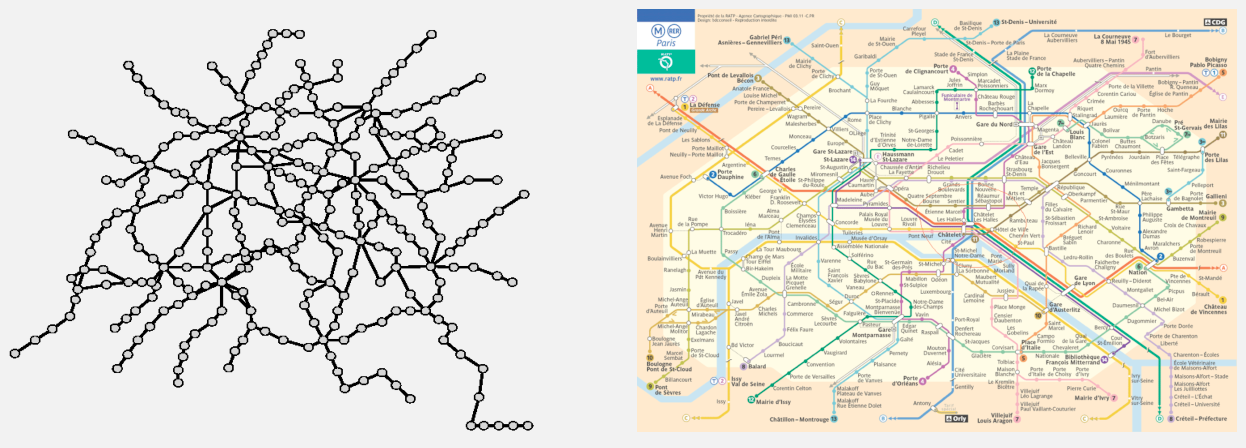
\includegraphics[width=\textwidth]{img/exemplos_grafos.png}
    \caption{Fonte: \cite{sedgewick2014algorithms}}
  \end{figure}

\end{frame}

\begin{frame}
  \frametitle{Grafos}
  
  \tcb{Por que estudar grafos e seus algoritmos?}
  \begin{itemize}
    \item Milhares de aplicações práticas;
    \item Vários algoritmos conhecidos;
    \item Abstrações interessantes e úteis;
    \item Campo desafiador da Ciência da Computação e da Matemática Discreta.
  \end{itemize}

\end{frame}

\begin{frame}
  \frametitle{Fronteiras entre os estados Brasileiros}

  \begin{figure}[h]
    \centering
    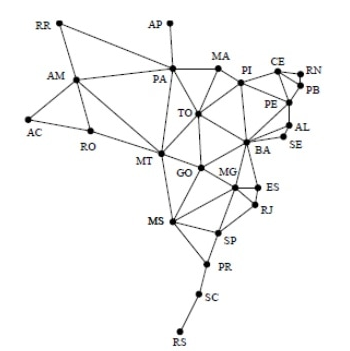
\includegraphics[width=.5\textwidth]{img/estados.png}
  \end{figure}
  
\end{frame}

\begin{frame}
  \frametitle{10 milhões de amizades no Facebook}

  \begin{figure}[h]
    \centering
    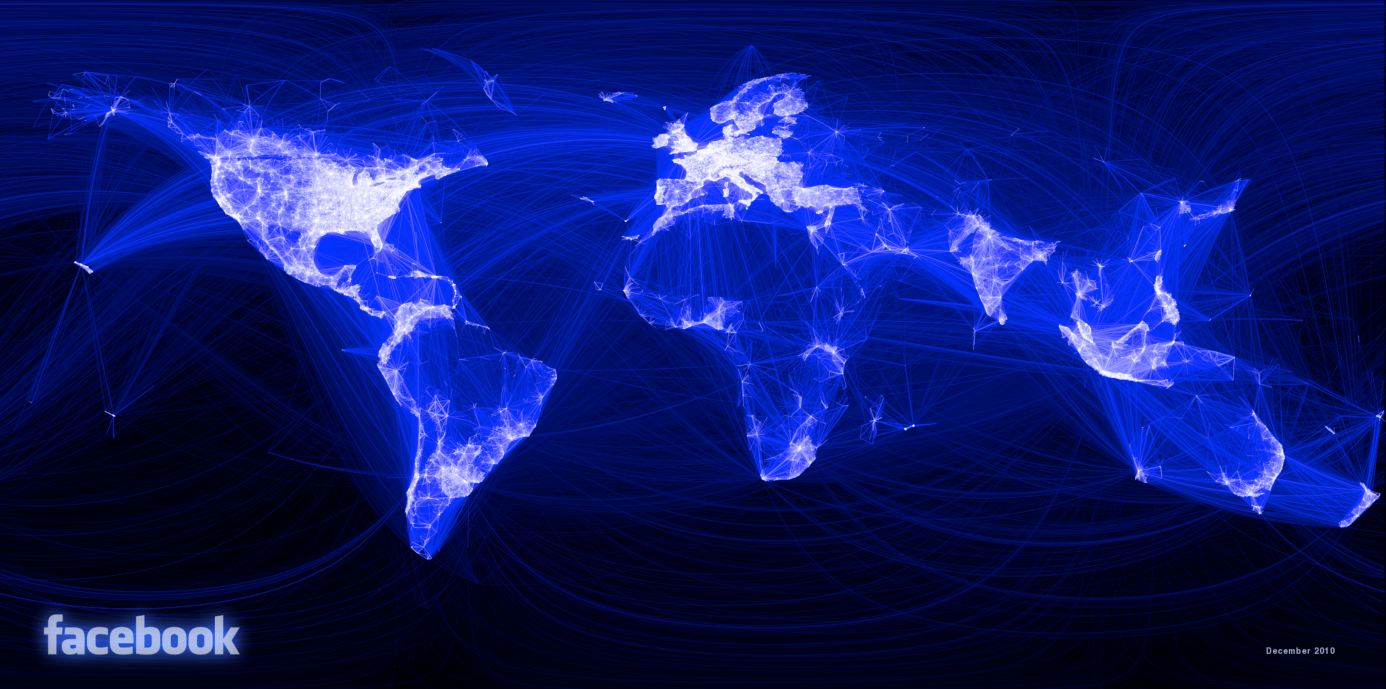
\includegraphics[width=\textwidth]{img/facebook.png}
    \caption{Fonte: \cite{sedgewick2014algorithms}}
  \end{figure}

\end{frame}

\begin{frame}
  \frametitle{Exemplos}

  \begin{table}[]
    \centering
    \scriptsize
    \begin{tabular}{@{}ccc@{}}
      \toprule
      Grafo & Vértice & Aresta \\ 
      \midrule
      Comunicação & telefone, computador & cabo de fibra óptica, cabo de rede  \\  
      Circuito & porta, registro, processador  & fio, filamento \\
      Financeiro & moeda, ações & transação \\
      Transporte & interseção  & rua  \\
      Jogos &  posição do tabuleiro & movimento válido  \\
      Relacionamento social &  pessoa & amizade \\
      Rede neural & neurônio  & sinapse \\
      Rede proteica & proteína & interação proteína-proteína \\
      Molécula & átomo & ligação \\
      \bottomrule
    \end{tabular}
  \end{table}
\end{frame}

\begin{frame}
  \frametitle{Terminologia de Grafos}

  \tcb{Caminho} Sequência de vértices conectados por arestas.

  \tcb{Ciclo} Caminho em que o primeiro vértice o último são o mesmo.

  Dois vértices são \tcr{conectados} se existe um caminho entre eles.
  
  \begin{figure}[h]
    \centering
    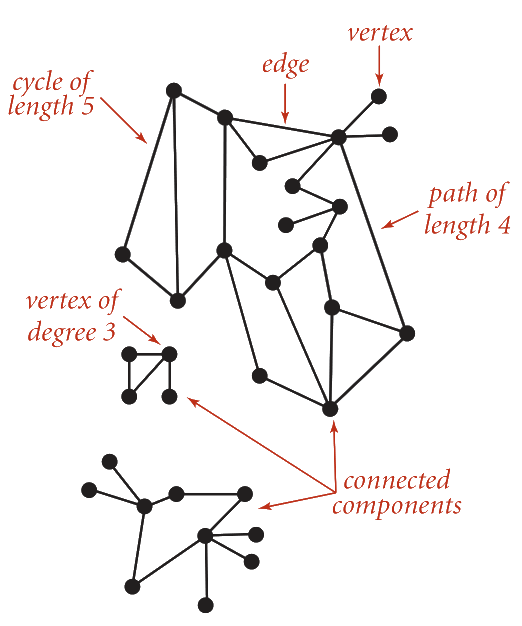
\includegraphics[width=.4\textwidth]{img/terminologia.png}
    \caption{Fonte: \cite{sedgewick2014algorithms}}
  \end{figure}

\end{frame}

\begin{frame}
  \frametitle{Alguns problemas com grafos}

  \begin{table}[]
    \centering
    \scriptsize
    \begin{tabular}{@{}cc@{}}
      \toprule
      Problema & Descrição \\ 
      \midrule
      Caminho s-t & \textit{Existe um caminho entre s e t?} \\  
      Menor caminho s-t & \textit{Qual o menor caminho entre s e t?} \\  
      Ciclo & \textit{Existe um ciclo no grafo?} \\
      Ciclo Euleriano & \textit{Existe um ciclo que usa cada aresta exatamente uma vez?} \\
      Ciclo Hamiltoniano & \textit{Existe um ciclo que usa cada vértice exatamente uma vez?} \\
      Conectividade & \textit{Existe um caminho para conectar todos os vértices?} \\
      Biconectividade & \textit{Existe um vértice que, se removido, desconecta o grafo?} \\
      Planaridade & \textit{É possível desenhar o grafo em um plano sem sobrepor arestas?} \\
      Isomorfismo & \textit{Duas listas de adjacências representam o mesmo grafo?} \\
      \bottomrule
    \end{tabular}
  \end{table}

  \tcb{Pergunta} Quais desses problemas são fáceis? Difíceis? Intratáveis?
\end{frame}

\section{Representação}

\begin{frame}
  \frametitle{Representação gráfica}

  Grafos podem ser representados graficamente e gerar intuições sobre a sua estrutura.

  \begin{figure}[h]
    \centering
    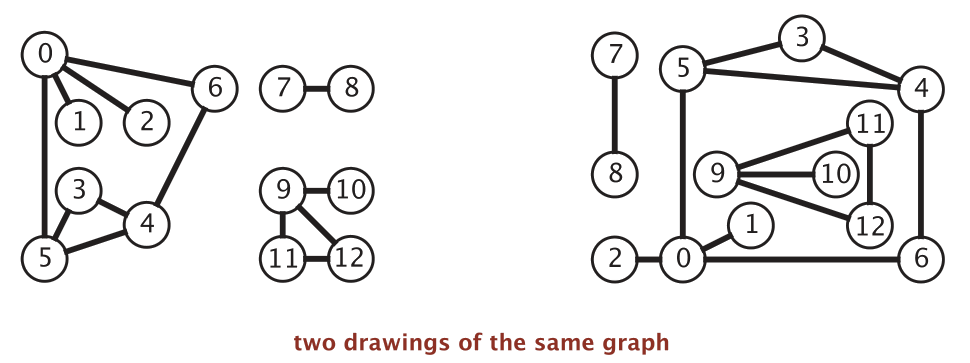
\includegraphics[width=\textwidth]{img/repr_grafica.png}
    \caption{Fonte: \cite{sedgewick2014algorithms}}
  \end{figure}

  \tcb{Importante} Intuições podem enganar.

\end{frame}
  
\begin{frame}
  \frametitle{Vértices}

  \begin{itemize}
    \item Utilizaremos valores inteiros para nomear os vértices;
    \item Aplicações reais podem converter nomes e números com tabelas de símbolos.
  \end{itemize}

  \begin{figure}[h]
    \centering
    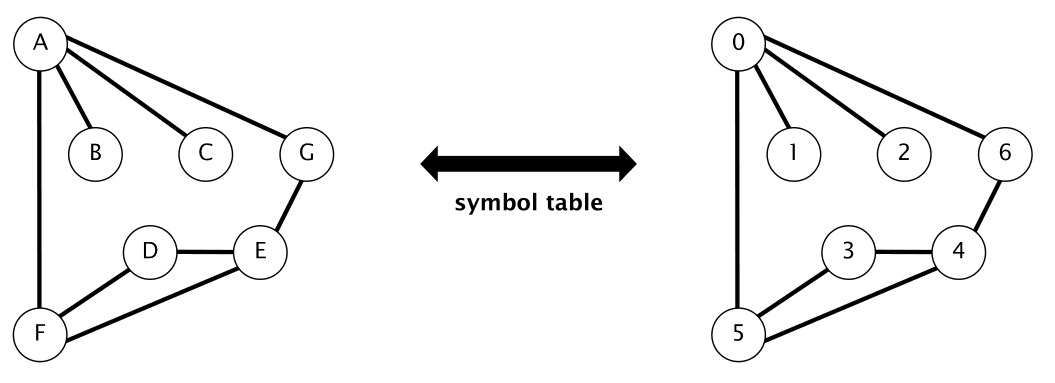
\includegraphics[width=\textwidth]{img/repr_vertices.png}
    \caption{Fonte: \cite{sedgewick2014algorithms}}
  \end{figure}

\end{frame}
  
\begin{frame}
  \frametitle{Anomalias}

  Consideraremos os itens na figura abaixo como anomalias. Entretanto, em algumas aplicações, eles podem ser considerados importantes.

  \begin{figure}[h]
    \centering
    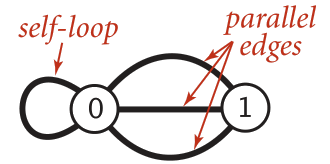
\includegraphics[width=.3\textwidth]{img/anomalias.png}
    \caption{Fonte: \cite{sedgewick2014algorithms}}
  \end{figure}

\end{frame}

\begin{frame}
  \frametitle{Representação Computacional}

  Para representar a estrutura de dados \tcb{Grafos} podemos considerar 3 opções:

  \begin{enumerate}
    \item Conjunto de arestas;
    \item Matriz de adjacências;
    \item Lista de adjacências;
  \end{enumerate}

\end{frame}

\begin{frame}
  \frametitle{Conjunto de arestas}

  Mantém um conjunto de arestas (lista ligada ou array).
  
  \begin{figure}[h]
    \centering
    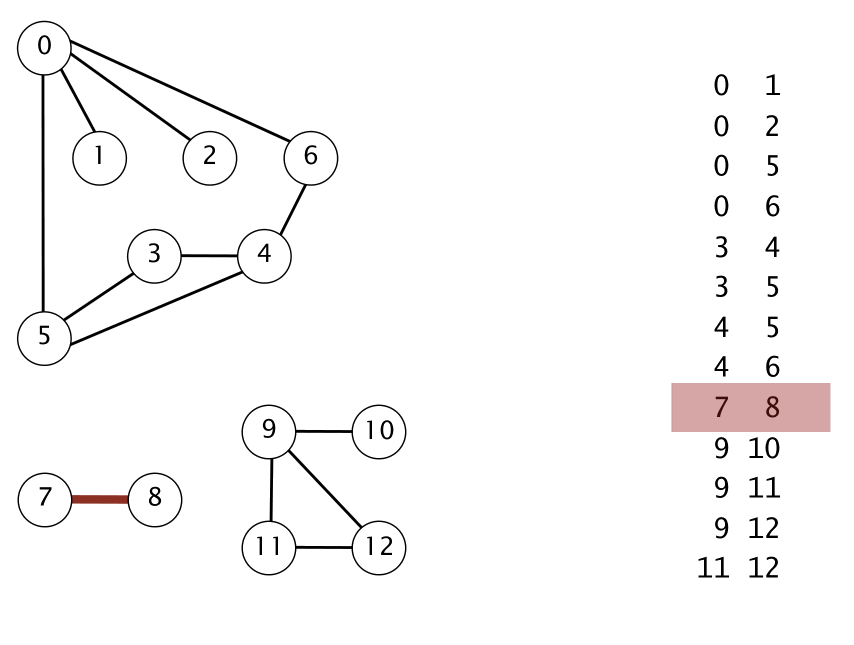
\includegraphics[width=.7\textwidth]{img/conj_de_arestas.png}
    \caption{Fonte: \cite{sedgewick2014algorithms}}
  \end{figure}

  \tcb{Q.} Quanto custa para iterar sobre todos os vértices adjacentes a $v$?

\end{frame}

\begin{frame}
  \frametitle{Matriz de Adjacências}

  Mantém uma matriz bidimensional de V por V booleanos;

  Para cada aresta $v-w$ no grafo:~\small \texttt{adj[v][w] = adj[w][v] = true}.

  \begin{figure}[h]
    \centering
    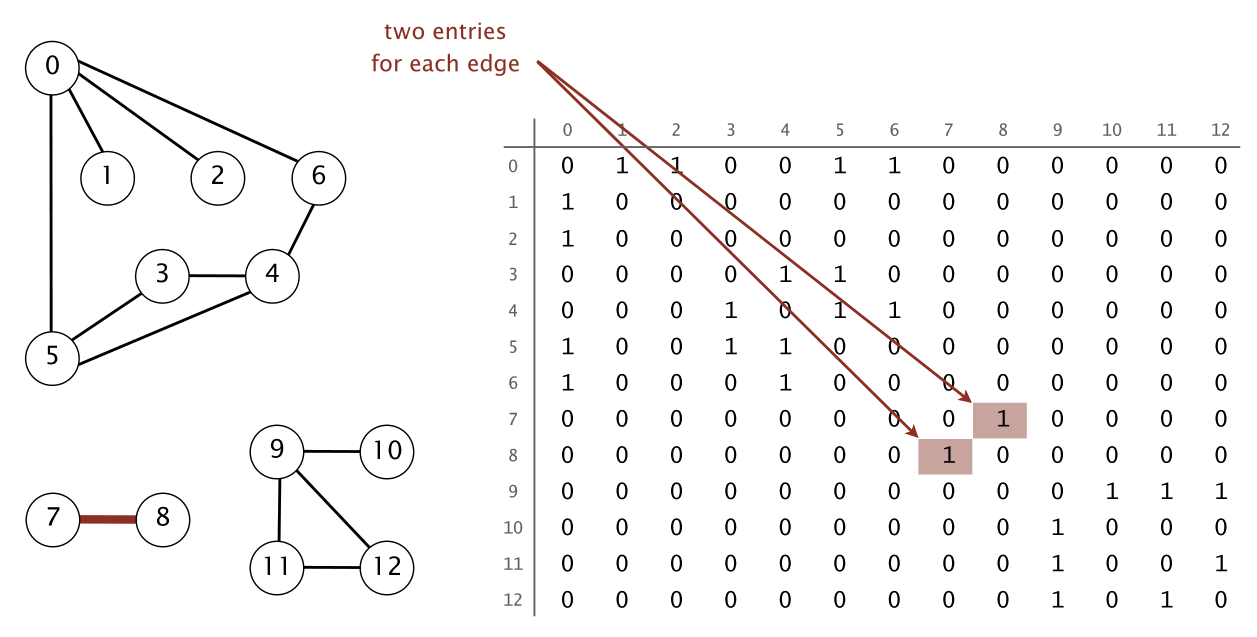
\includegraphics[width=.8\textwidth]{img/matriz_de_adjacencias.png}
    \caption{Fonte: \cite{sedgewick2014algorithms}}
  \end{figure}

  \tcb{Q.} Quanto custa para iterar sobre todos os vértices adjacentes a $v$?

\end{frame}
\begin{frame}
  \frametitle{Lista de Adjacências}

  Mantém um array de listas com as arestas de cada vértice.
  
  \begin{figure}[h]
    \centering
    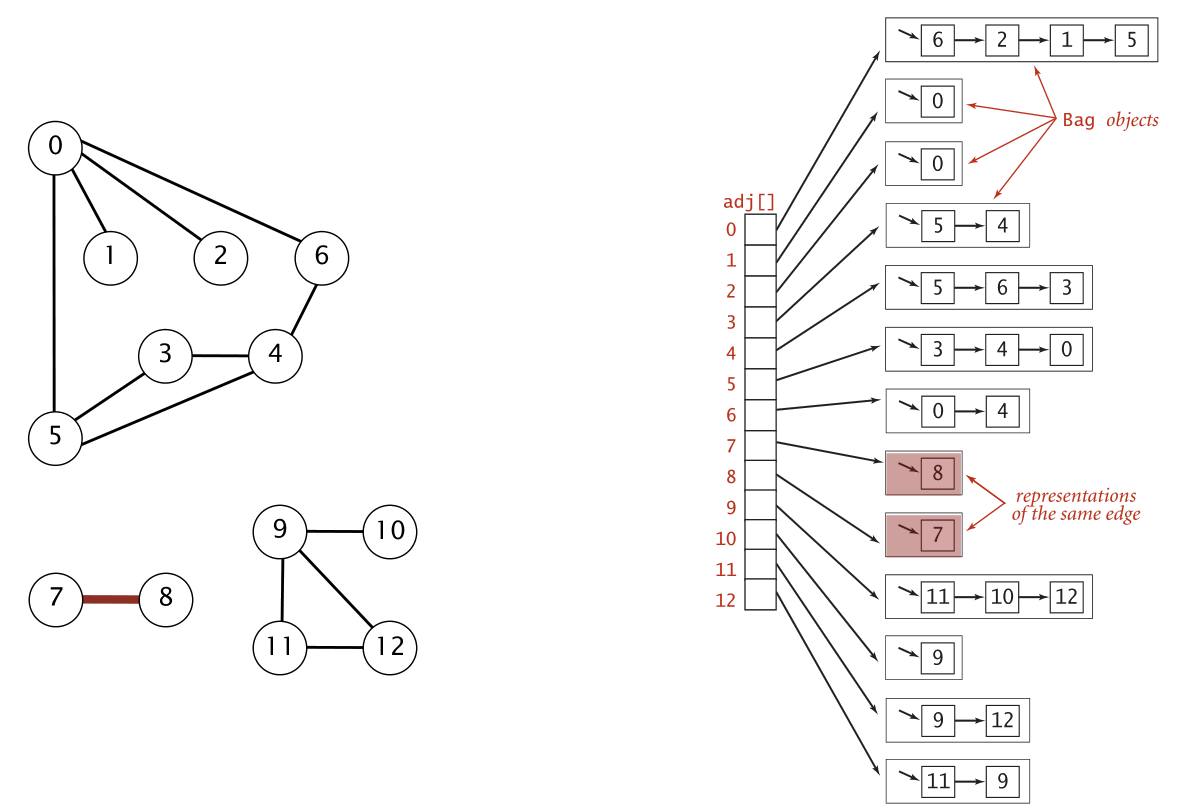
\includegraphics[width=.8\textwidth]{img/lista_de_adjacencias.png}
    \caption{Fonte: \cite{sedgewick2014algorithms}}
  \end{figure}

  \tcb{Q.} Quanto custa para iterar sobre todos os vértices adjacentes a $v$?

\end{frame}

\begin{frame}
  \frametitle{Qual a melhor representação?}
  
  \pause

  \tcb{Na prática:} Utilizar \textbf{lista de adjacências}:
  \begin{itemize}
    \item Algoritmos são geralmente baseados na iteração sobre os vértices adjacentes a $v$;
    \item Grafos de problemas reais tendem a ser \tcr{esparsos}:
      \begin{itemize}
        \item Número alto de vértices mas com \tcr{grau médio} pequeno.
      \end{itemize}
  \end{itemize}

  \begin{figure}[h]
    \centering
    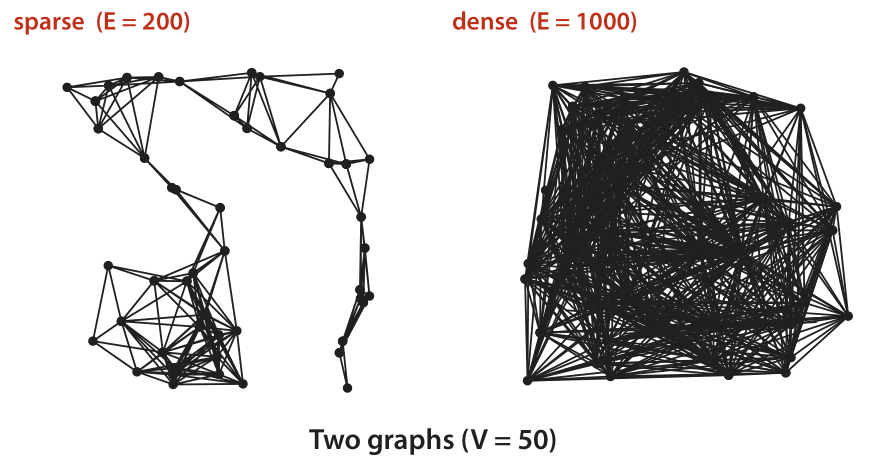
\includegraphics[width=.8\textwidth]{img/esparso.png}
    \caption{Fonte: \cite{sedgewick2014algorithms}}
  \end{figure}

\end{frame}

\renewcommand{\thefootnote}{*}

\begin{frame}
  \frametitle{Comparação entre Representações}

  \begin{table}[]
    \centering
    \scriptsize
    \begin{tabular}{c|c|c|c|c}
      \toprule
      \textbf{Representação} & 
      \textbf{Espaço} & 
      \textbf{Adicionar aresta} & 
      \Centerstack[c]{\textbf{Aresta entre}\\ \textbf{$v$ e $w$?}} &
      \Centerstack[c]{\textbf{Iterar sobre}\\ \textbf{os vizinhos}\\ \textbf{de $v$?}}\\ 
      \midrule
      Conjunto de arestas & $E$ & 1 & $E$ & $E$ \\
      Matriz de Adjacências & $V^2$ & 1\footnote[frame]{Não permite arestas paralelas} & 1 & $V$\\
      Lista de Adjacências & $E+V$ & 1 & $grau(v)$ & $grau(v)$\\
      \bottomrule
    \end{tabular}
  \end{table}

\end{frame}

\section{Implementação}

\begin{frame}[fragile]
  \frametitle{Estrutura para Listas de Adjacências}

\begin{minted}[frame=lines,framesep=2mm,baselinestretch=1,fontsize=\small,linenos]{c}
typedef struct node *link;
struct node {
  int w;               // destination node of edge
  link next;           // next element in adjacency list
};

struct graph {
  int V;               // number of vertices
  int E;               // number of edges
  link *adj;           // adjacency list
};
typedef struct graph *Graph;
typedef struct { int v; int w; } Edge;
\end{minted}

\end{frame}

\begin{frame}[fragile]
  \frametitle{Criação de um Grafo}

\begin{minted}[frame=lines,framesep=2mm,baselinestretch=1,fontsize=\normalsize,linenos]{c}
Graph GRAPHinit(int V) {
  int v;
  Graph G = malloc(sizeof *G);
  G->V = V; G->E = 0;
  G->adj = malloc(V * sizeof(*G->adj));
  if (G->adj == NULL){
     fprintf(stderr, "Out of memory in GRAPHinit()\n");
     exit(EXIT_FAILURE);
  }

  for (v = 0; v < V; v++) G->adj[v]  = NULL;

  return G;
}
\end{minted}
\end{frame}

\begin{frame}[fragile]
  \frametitle{Inserção de Aresta}

\begin{minted}[frame=lines,framesep=2mm,baselinestretch=1,fontsize=\normalsize,linenos]{c}
void GRAPHinsertE(Graph G, Edge e) {
  int v = e.v;
  int w = e.w;
  G->adj[v] = NEW(w, G->adj[v]);
  G->adj[w] = NEW(v, G->adj[w]); 
  G->E++;
}
\end{minted}

\end{frame}

\section{Busca em Profundidade}

\begin{frame}
  \frametitle{Exploração em Labirintos}

  \tcb{Grafo de um Labirinto:}
  \begin{itemize}
    \item Vértice = interseção;
    \item Aresta = passagem.
  \end{itemize}
  
  \begin{figure}[h]
    \centering
    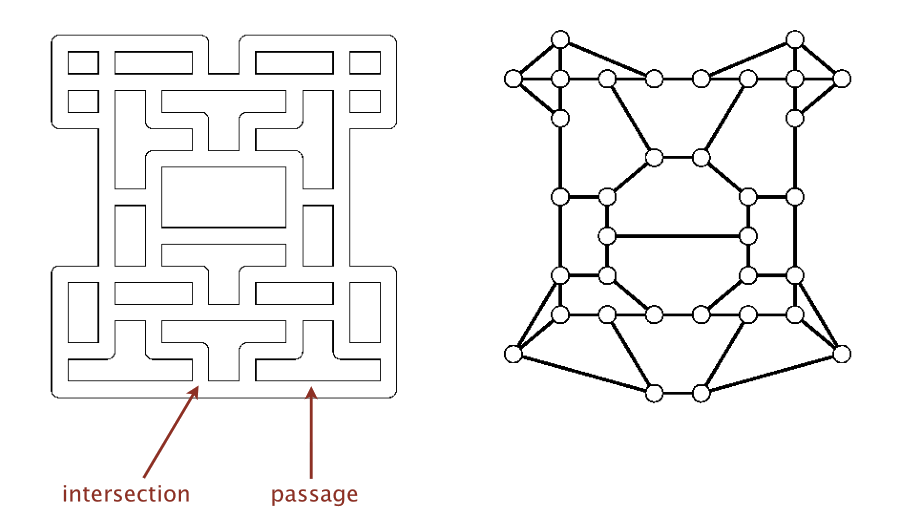
\includegraphics[width=.6\textwidth]{img/grafo_labirinto.png}
    \caption{Fonte: \cite{sedgewick2014algorithms}}
  \end{figure}

  \tcb{Objetivo} Explorar cada interseção (vértice) do labirinto.

\end{frame}

\begin{frame}
  \frametitle{Exploração em Labirintos}

  \tcb{Algoritmo possível}
  \begin{itemize}
    \item Desenrolar um novelo de lã atrás de você;
    \item Assim, marcamos cada interseção visitada e cada passagem visitada;
    \item Voltar pelo fio de lã quando ficar sem saída para última interseção com passagens não visitadas.
  \end{itemize}
  
  \begin{figure}[h]
    \centering
    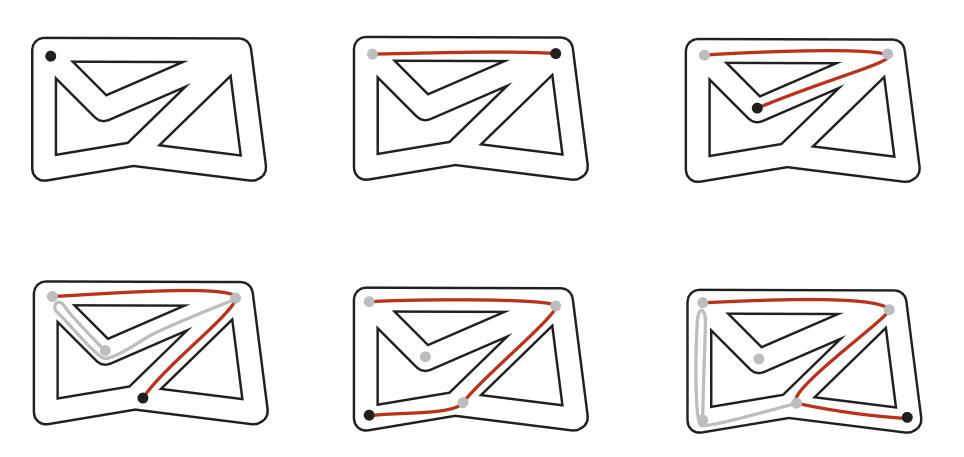
\includegraphics[width=.6\textwidth]{img/alg_labirinto.png}
    \caption{Fonte: \cite{sedgewick2014algorithms}}
  \end{figure}

\end{frame}

\begin{frame}
  \frametitle{Labirinto Fácil}

  \begin{figure}[h]
    \centering
    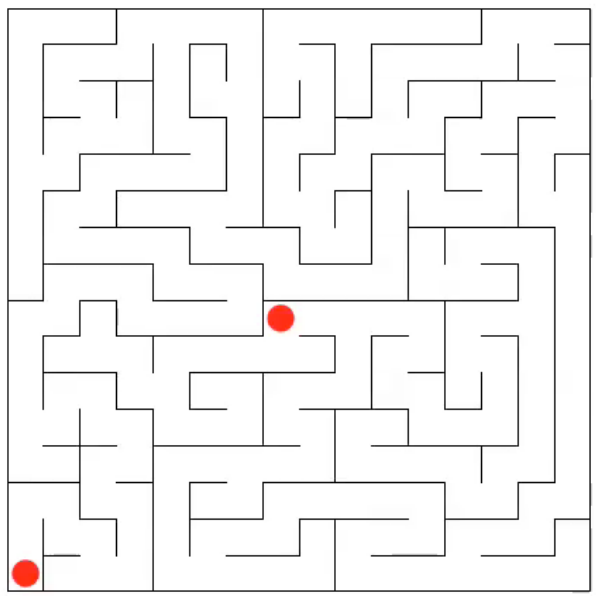
\includegraphics[width=.6\textwidth]{img/labirinto_facil.png}
    \caption{Fonte: \cite{sedgewick2014algorithms}}
  \end{figure}

\end{frame}

\begin{frame}
  \frametitle{Labirinto Difícil}

  \begin{figure}[h]
    \centering
    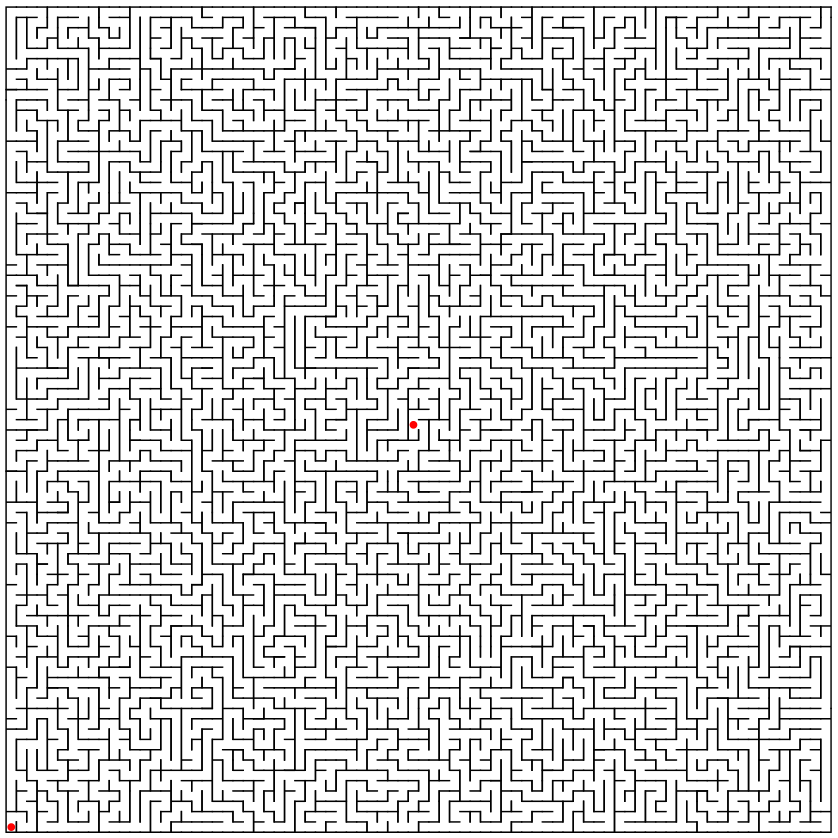
\includegraphics[width=.6\textwidth]{img/labirinto_dificil.png}
    \caption{Fonte: \cite{sedgewick2014algorithms}}
  \end{figure}

\end{frame}

\begin{frame}
  \frametitle{Busca em Profundidade}

  \tcb{Objetivo} Percorrer o grafo sistematicamente.

  \tcb{Ideia} Imitar a exploração de labirintos (pilha de funções como novelo de lã).


\begin{algorithm}[H]
\DontPrintSemicolon
\SetKwProg{Fn}{def}{\string:}{}
\Fn{DFS(visitar um vertice v)}
{
  Marcar v como visitado\;
  Recursivamente visitar todos os vizinhos não marcados de v\;
}
\caption{Depth-first search (Busca em Profundidade)}
\end{algorithm}


  \tcb{Aplicações Típicas:} 
  \begin{itemize}
    \item Encontrar todos os vértices conectados a um dado vértice;
    \item Encontrar um caminho entre dois vértices.
  \end{itemize}
  
\end{frame}

\begin{frame}
  \frametitle{Exemplo Busca em Profundidade}

  \begin{figure}[h]
    \centering
    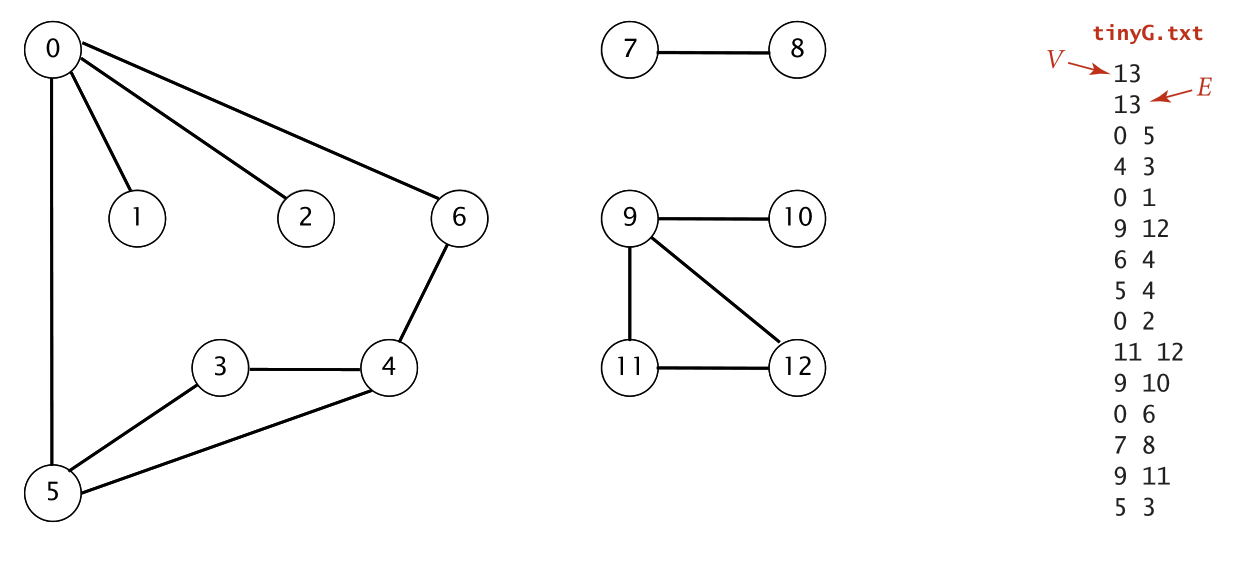
\includegraphics[width=.8\textwidth]{img/ex_dfs.png}
    \caption{Fonte: \cite{sedgewick2014algorithms}}
  \end{figure}

  \tcb{Estruturas auxiliares}
  \begin{itemize}
    \item Array \texttt{marked[]} para marcar vértices visitados; 
    \item Array \texttt{edgeTo[]} para salvar caminhos:
    \begin{itemize}
      \item \texttt{(edgeTo[w] == v)} significa que a aresta $v-w$ foi utilizada para visitar $w$ pela primeira vez.
    \end{itemize}
  \end{itemize}

\end{frame}

\begin{frame}
  \frametitle{Exemplo Busca em Profundidade}
  
  \multiinclude[<+->][format=png, graphics={width=\textwidth}]{img/dfs/dfs}
\end{frame}

\begin{frame}
  \frametitle{Exemplo Busca em Profundidade}

  \begin{figure}[h]
    \centering
    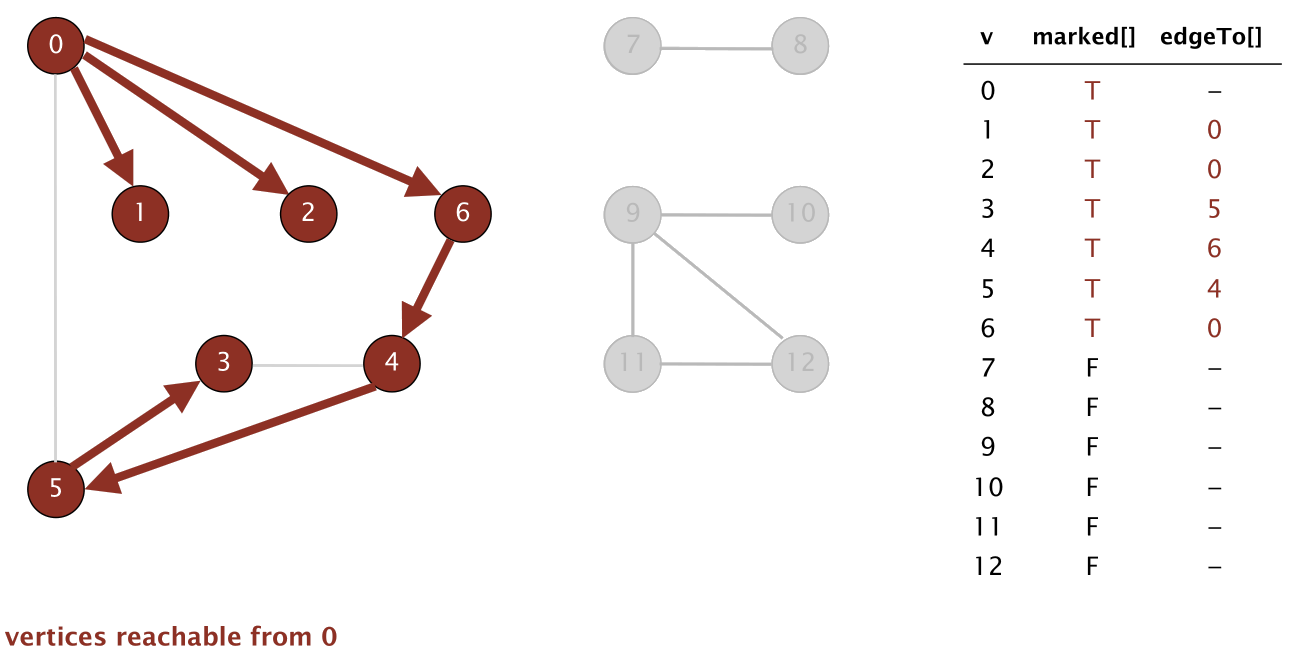
\includegraphics[width=.8\textwidth]{img/ex_dfs_2.png}
    \caption{Fonte: \cite{sedgewick2014algorithms}}
  \end{figure}

  Depois da DFS é possível
  \begin{itemize}
    \item Verificar se o vértice $v$ é conectado a outro vertice $s$ em tempo constante; 
    \item Encontrar caminho o caminho $v-s$ em tempo proporcional ao comprimento do caminho.
  \end{itemize}

\end{frame}

\section{Busca em Largura}

\begin{frame}
  \frametitle{Ideia}

  Percorrer o grafo seguindo uma \tcb{fila} e não uma \tcr{pilha} como na busca em profundidade.
  
\begin{algorithm}[H]
\DontPrintSemicolon
\SetKwProg{Fn}{def}{\string:}{}
\Fn{BFS(visitar um vertice v)}
{
  Inserir $v$ na fila\;
  \While{Fila não vazia}{
    Remover $v$ da fila\;
    Inserir na fila todos os vizinhos não marcados de $v$ e marcá-los\;
  }
}
\caption{Breadth-first search (Busca em Largura)}
\end{algorithm}

\end{frame}

\begin{frame}
  \frametitle{Exemplo Busca em Largura}

  \begin{figure}[h]
    \centering
    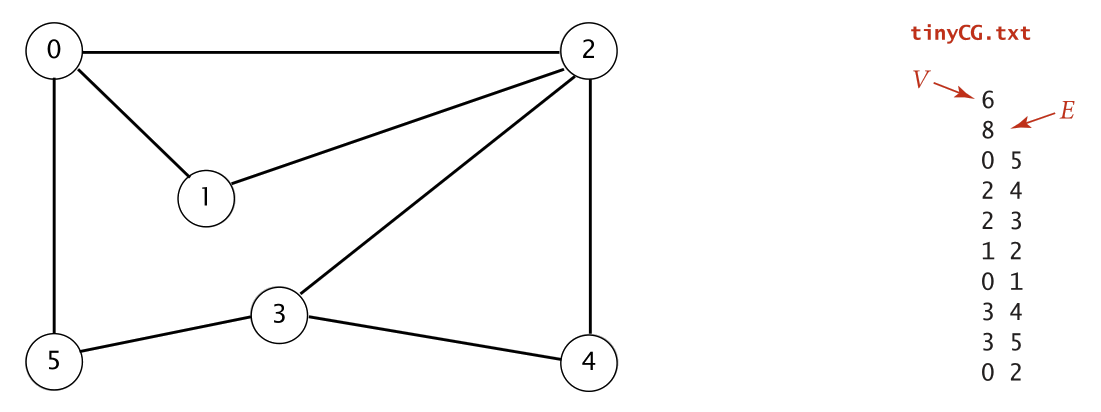
\includegraphics[width=.8\textwidth]{img/ex_bfs.png}
    \caption{Fonte: \cite{sedgewick2014algorithms}}
  \end{figure}

  \tcb{Estruturas auxiliares}
  \begin{itemize}
    \item Array \texttt{distTo[]} para distâncias a partir de $v$;
    \item Array \texttt{edgeTo[]} para salvar caminhos:
    \begin{itemize}
      \item \texttt{(edgeTo[w] == v)} significa que a aresta $v-w$ foi utilizada para visitar $w$ pela primeira vez.
    \end{itemize}
  \end{itemize}

\end{frame}

\begin{frame}
  \frametitle{Exemplo Busca em Largura}
  
  \multiinclude[<+->][format=png, graphics={width=\textwidth}]{img/bfs/bfs}
\end{frame}

\begin{frame}
  \frametitle{Exemplo Busca em Largura}

  \begin{figure}[h]
    \centering
    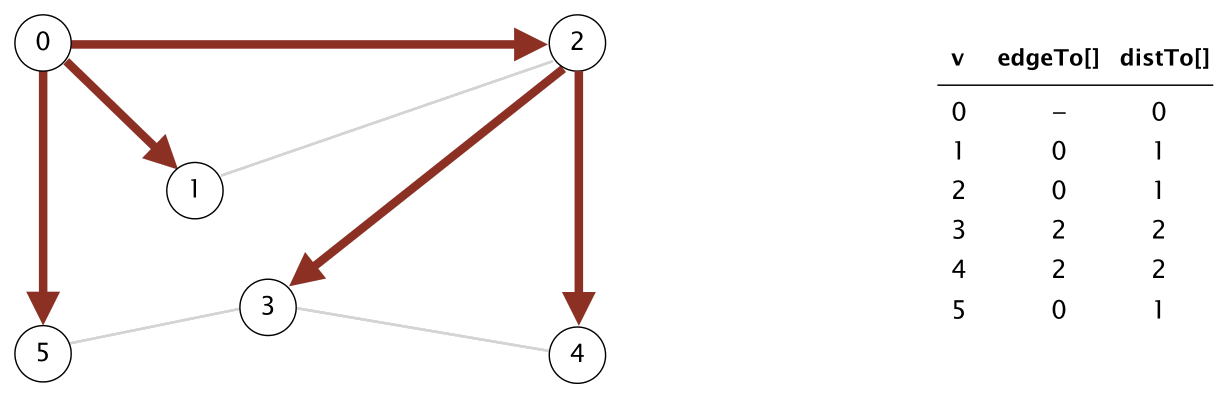
\includegraphics[width=.8\textwidth]{img/ex_bfs_2.png}
    \caption{Fonte: \cite{sedgewick2014algorithms}}
  \end{figure}

  Com a BFS é possível
  \begin{itemize}
    \item Determinar o menor caminho entre $v$ e outros vértices em tempo proporcional a $E+V$.
  \end{itemize}

\end{frame}

\begin{frame}
  \frametitle{Cálculo de Menor Caminho por Busca em Largura}

  \begin{figure}[h]
    \centering
    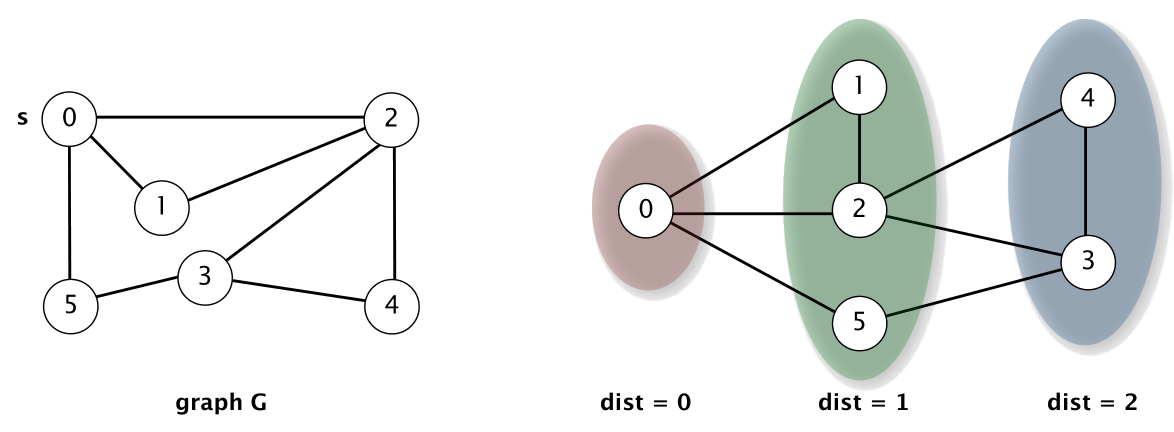
\includegraphics[width=.8\textwidth]{img/ex_bfs_3.png}
    \caption{Fonte: \cite{sedgewick2014algorithms}}
  \end{figure}

\end{frame}

\section{Componentes Conexas}

\begin{frame}
  \frametitle{Definição}

  A relação ``é conectado à'' é uma relação de equivalência:
  \begin{itemize}
    \item Reflexiva: $v$ é conectado à $v$;
    \item Simétrica: se $v$ é conectado à $w$, então $w$ é conectado à $v$;
    \item Transitiva: se $v$ é conectado à $w$ e $w$ é conectado à $x$, então $v$ é conectado à $x$;
  \end{itemize}

  \tcb{Definição} Uma \tcr{componente conexa} é um conjunto máximo de vértices (não é possível adicionar mais nenhum ao conjunto).

\end{frame}

\begin{frame}
  \frametitle{Exemplo}

  \begin{figure}[h]
    \centering
    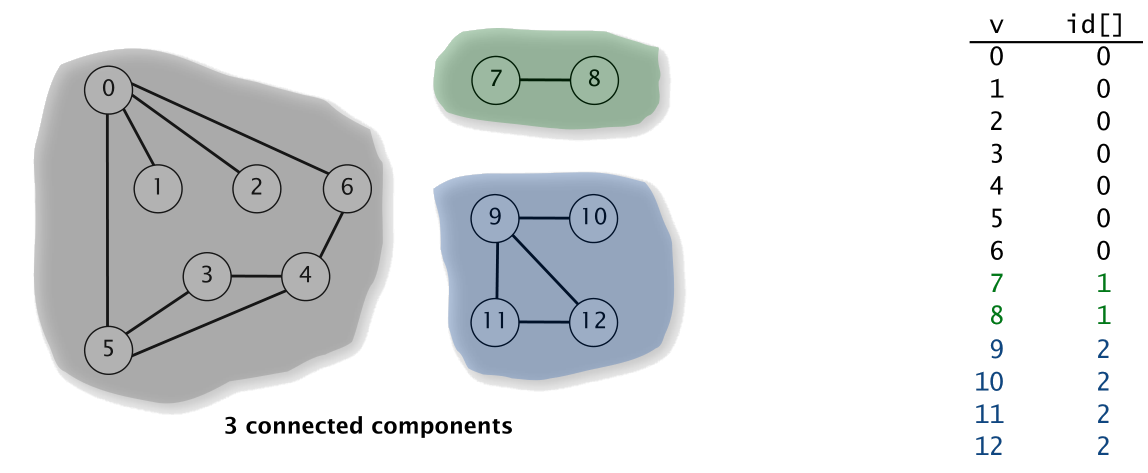
\includegraphics[width=.8\textwidth]{img/ex_cc.png}
    \caption{Fonte: \cite{sedgewick2014algorithms}}
  \end{figure}

\end{frame}

\begin{frame}
  \frametitle{Exemplo}

  \begin{figure}[h]
    \centering
    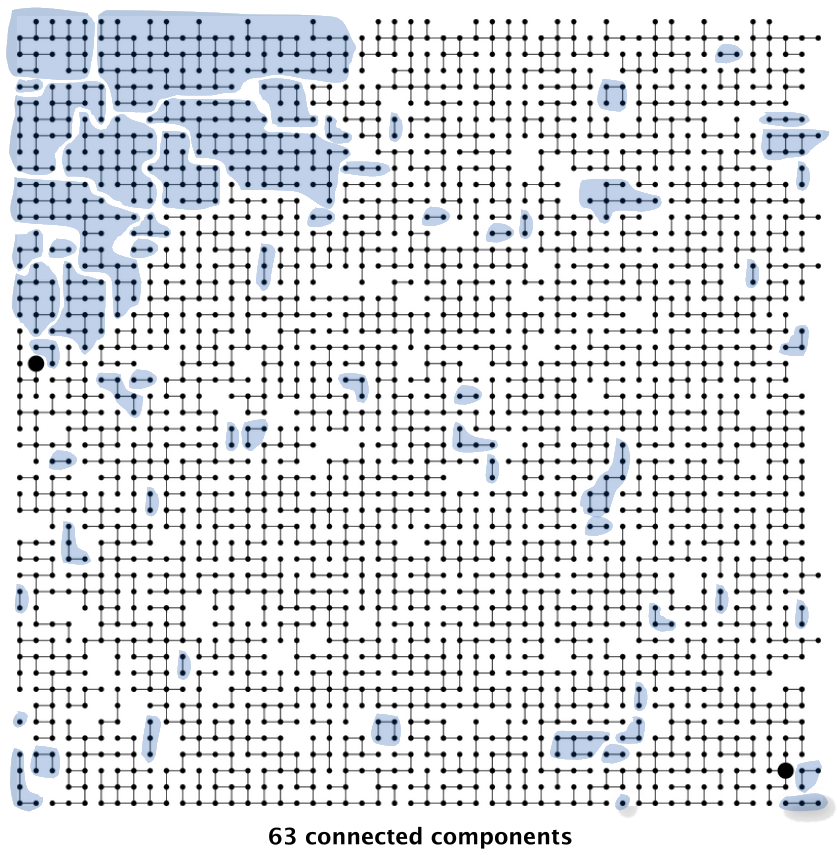
\includegraphics[width=.7\textwidth]{img/ex_cc_2.png}
    \caption{Fonte: \cite{sedgewick2014algorithms}}
  \end{figure}

\end{frame}

\section{Conclusão}

\begin{frame}
  \frametitle{Problemas de Grafos e suas Buscas}

  \begin{figure}[h]
    \centering
    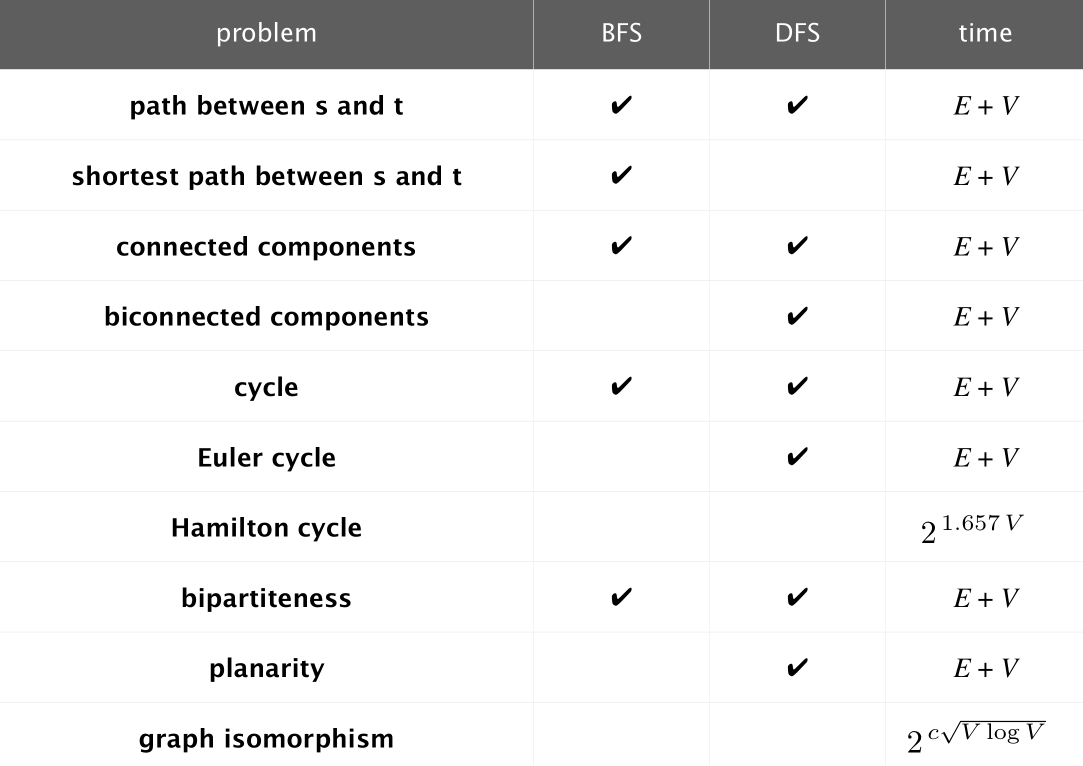
\includegraphics[width=.7\textwidth]{img/problemas_buscas.png}
    \caption{Fonte: \cite{sedgewick2014algorithms}}
  \end{figure}

\end{frame}

\begin{frame}
  \frametitle{Referências utilizadas na apresentação}
  \bibliography{referencias}
\end{frame}
% ==========================================

\end{document}
